\documentclass{cours}
\usepackage{pgfplots}
\usepackage{multicol}
\usepackage{amssymb}
\usepackage{fontawesome}
\usetikzlibrary {decorations.text}
\usepackage{mhchem}
\begin{document}


\setcounter{chapter}{19}
\chapter{Diagrammes potentiel-pH}

\section{Diagramme potentiel-pH de l'eau}%
\label{sec:diagramme_potentiel_ph_de_l_eau}

L'eau intervient dans les couples redox suivants:
\begin{itemize}
  \item \ce{O2 / H2O} de potentiel standard $E^\circ_{\ce{O2 / H2O}}=\SI{1.23}{\volt}$ et de demi-équation
  \begin{equation}
    \ce{O2 + 4H+ + 4e- <=> 2H2O}\,;
  \end{equation}
  \item \ce{H2O /H2} de potentiel standard $E^\circ_{\ce{H2O / H2}}=\SI{0}{\volt}$ et de demi-équation :
  \begin{equation}
    \ce{H2O + 2H+ + 2e- <=>H2 + H2O}\, .
  \end{equation}
\end{itemize}
En appliquant la formule de Nernst à ces deux couples à \SI{25}{\celsius}, on peut exprimer leur potentiel en fonction du pH de la solution :
  \begin{equation}
  E_{\ce{O2 / H2O}} = E_{\ce{O2 / H2O}}^\circ + \frac{\num{0.06}}{4}\log\left( \left(\frac{[\ce{H+}]}{\cz}\right)^4  \frac{p(\ce{O2})}{p^\circ}\right) = E_{\ce{O2 / H2O}}^\circ - \num{0.06}\pH
  \end{equation}
  et
  \begin{equation}
  E_{\ce{H2O / H2}} = E_{\ce{H2O / H2}}^\circ + \frac{\num{0.06}}{2}\log\left( \left(\frac{[\ce{H+}]}{\cz}\right)^2  \frac{p^\circ}{p(\ce{H2})}\right) = E_{\ce{H2O / H2}}^\circ - \num{0.06}\pH
  \end{equation}
Pour obtenir ces deux équations, on a aussi supposé que les pressions de \ce{O2} et de $\ce{H2}$ étaient égales à $p^\circ$. C'est un choix arbitraire de \emph{pression de travail} , on aurait pu en faire un autre mais ça ne changerait pas fondamentalement le principe de la méthode.

Le résultat important est que le potentiel de ces deux couples dépend du pH de la solution. On peut donc tracer un graphique qui représente ces deux potentiels en fonction du pH, et y faire figurer les domaines de stabilité des différentes espèces chimiques
\begin{center}
  \begin{tikzpicture}
    \begin{axis}[
    domain=0:14,
      xmin=0,
      xmax=14,
      ymax=2,
      ymin=-1,
      extra y ticks={1.23},
      xlabel=pH,
      ylabel=E(V),
      clip=false,
    ]
      \draw[ultra thick, gray!30] (axis cs:10, -1) -- (axis cs:10,2);
      \addplot[thick] {1.23-0.06*x} node[midway, below, sloped]{Domaine de stabilité de l'eau};
      \addplot[thick] {-0.06*x};
      \node at (axis cs:7, 1.5) {\ce{O2}};
      \node at (axis cs:7, -7*0.06+1.23/2) {\ce{H2O}}; 
      \node at (axis cs:7, -7*0.06-0.4) {\ce{H2}};
      \coordinate (A) at (axis cs:10,0);
    \end{axis}
  \begin{scope}[xshift=9cm, yshift=2cm]
  \draw[-latex] (0,0) -- (6,0) node[right]{$E$}; 
  \coordinate (F1) at ({6/3*(1-10*0.06)}, 0);
  \coordinate (F2) at ({6/3*(1+1.23-10*0.06)}, 0);
  \draw (F1) -- ++(0,0.5) node[below left]{\ce{H2}} coordinate(P1);
  \draw (F2) -- ++(0,0.5) coordinate (P2);
  \draw ($(P1)!0.5!(P2)$) node[below]{\ce{H2O}};
  \draw ($(P2)+(1.5, 0)$) node[below]{\ce{O2}};
  \draw[gray!30, thick, -latex] (A) to[out=0, in=180] (0,0);
  \end{scope}
  \end{tikzpicture}
  \captionof{figure}{Diagramme potentiel-pH de l'eau et diagramme de prédominance des différentes espèces à $\pH=10$. Le diagramme potentiel-pH est la représentation des diagrammes de prédominance à tous les pH possibles.}
\end{center}

\section{Diagramme potentiel-pH du fer}%
\label{sec:diagramme_potentiel_ph_du_fer}
Le diagramme potentiel-pH du fer est un peu plus compliqué à construire que celui de l'eau. C'est surtout du au fait que l'élément fer intervient dans beaucoup plus de couples que l'eau. Nous allons procéder par étapes.

\subsection{Conventions, diagramme de situation}%
\label{sub:conventions_diagramme_de_situation}

Par convention, on considérera que, sur une frontière, la concentrationde toutes les espèces diluées intervenant dans le diagramme est égale à la \emph{concentration de travail} $c_t=\SI{e-2}{\mol\per\litre}$. (Il peut exister d'autres conventions de tracé, par exemple on peut donner la concentration totale en espèces dissoutes, ou la concentration totale en élément dissout)   

On commence par recenser toutes les espèces chimiques du fer rencontrées en solution aqueuse : \ce{Fe(s)}, \ce{Fe^2+(aq)}, \ce{Fe^3+(aq)}, \ce{FE(OH)2(s)}, \ce{Fe(OH)3(s)}.

Puis on les classe par nombre d'oxydation pour l'élément fer :
\begin{center}
  \begin{tabular}{ll}
    \toprule
    nombre d'oxydation & espèces \\
    \midrule
    +III & \ce{Fe^3+}, \ce{Fe(OH)3}\\
    +II & \ce{Fe^2+}, \ce{Fe(OH)2}\\
    0 & \ce{Fe}\\
    \bottomrule
  \end{tabular}
\end{center}

On détermine les pH limites de précipitation des espèces solides :
\begin{itemize}
  \item Pour \ce{Fe(OH)3}, on a la réaction de dissolution :
  \begin{equation}
    \ce{Fe(OH)3 (s) <=> Fe^3+ + 3HO-}
  \end{equation}
  de produit de solubilité 
  \begin{equation}
    K_S = \frac{[\ce{Fe^3+}][\ce{HO-}]^3}{\cz^4} = \num{e-37}
  \end{equation}
  On rapelle que $[\ce{Fe^3+}] = c_t = \SI{e-2}{\mol\per\litre}$ ce qui donne
  \begin{equation}
    -\log(K_S) = -\log\left( \frac{c_t}{\cz} \right) -3\log \left( \frac{[\ce{HO-}]}{\cz} \right) \Leftrightarrow 37 = 2 + 3(14-\pH) \Leftrightarrow \pH=\num{2.3}
  \end{equation}

  \item Pour \ce{Fe(OH)2}, on a la réaction de dissolution :
  \begin{equation}
    \ce{Fe(OH)2 <=> Fe^2+ + 2HO-}
  \end{equation}
  de produit de solubilité
  \begin{equation}
    K_S = \frac{[\ce{Fe^2+}][\ce{HO-}]^2}{\cz^3}=10^{\num{-15.1}}
  \end{equation}
  De la même manière, on trouve un pH de précipitation de \num{7.5}.
\end{itemize}
On établit alors un \textbf{diagramme de situation} 
\begin{center}
  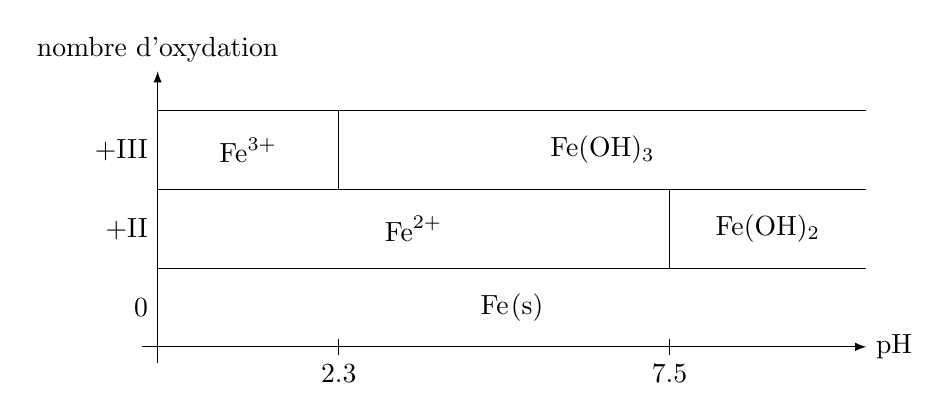
\begin{tikzpicture}
    \draw[-latex] (-0.2, 0) -- (9, 0) node[right]{pH};
    \draw[-latex] (0, -0.2) -- (0, 3.5) node[above]{nombre d'oxydation};
    \draw (2.3, -0.1) node[below](pH1){\num{2.3}} -- ++(0, 0.2);
    \draw (6.5, -0.1) node[below](pH1){\num{7.5}} -- ++(0, 0.2);
    \draw (0,1) -- (9, 1);
    \draw (0,2) -- (9, 2);
    \draw (0,3) -- (9, 3);
    \draw (4.5, 0.5) node {\ce{Fe(s)}};
    \draw (6.5, 1) -- ++(0,1);
    \draw (2.3, 2) -- ++(0,1);
    \draw (3.25, 1.5) node {\ce{Fe^2+}};
    \draw (7.75, 1.5) node {\ce{Fe(OH)2}};
    \draw (1.15, 2.5) node {\ce{Fe^3+}};
    \draw (5.65, 2.5) node {\ce{Fe(OH)3}};
    \draw (0, 0.5) node[left]{$0$}; 
    \draw (0, 1.5) node[left]{$+$II}; 
    \draw (0, 2.5) node[left]{$+$III}; 
  \end{tikzpicture}
\end{center}


Ce diagramme indique les positions relatives des frontières du diagramme E-pH. Il va falloir déterminer les équations de toutes les frontières horizontales.

\subsection{Équations des frontières}%
\label{sub:equations_des_frontieres}
\begin{itemize}
  \item \underline{\ce{Fe^2+ / Fe} : } 

  Demi-équation 
\begin{equation}
  \ce{Fe^2+ + 2e- <=> Fe}
\end{equation}
Formule de Nernst
  \begin{equation}
    E = E^\circ + \frac{\num{0.06}}{2}\underbrace{\log\left( \frac{[\ce{Fe^2+}]}{\cz}\right)}_{=-2} = -\num{0.44}-\num{0.06} = \SI{-0.50}{\volt} 
  \end{equation}
  Le potentiel ne dépend pas du pH, donc la frontière est \textbf{horizontale}.

\item \underline{\ce{Fe^2+ / Fe^3+}}

Demi-équation
\begin{equation}
  \ce{Fe^3+ + e- <=> Fe^2+}
\end{equation}
Formule de Nernst
\begin{equation}
E = E^\circ + \num{0.06} \log \left( \frac{[\ce{Fe^3+}}{\ce{Fe^2+}} \right) 
\end{equation}
Sur la frontière, on a $[\ce{Fe^2+}]=[\ce{Fe^3+}]$ et donc $E = E^\circ = \SI{0.77}{\volt}$. La frontière est horizontale.

  \item \underline{\ce{Fe(OH)2 / Fe} : } 

Demi-équation 
\begin{equation}
\ce{Fe(OH)2 + 2e- + 2H+ <=> Fe + 2H2O}
\end{equation}
Formule de Nernst
\begin{equation}
  E = E^\circ + \frac{\num{0.06}}{2}\log \left( \frac{[\ce{H+}]^2}{\cz^2} \right) = E^\circ -   \num{0.06}\pH
\end{equation}
La frontière est une droite de pente \SI{-0.06}{\volt}.

\item \underline{\ce{Fe(OH)3 /  Fe^2+} : }

Demi-équation
\begin{equation}
  \ce{Fe(OH)3 +  3H+ + e- <=> Fe^2+ + 3H2O}
\end{equation}
Formule de Nernst
\begin{equation}
  E = E^\circ + \frac{\num{0.06}}{1}\log \left( \frac{[\ce{H+}]^3}{[\ce{Fe^2+]\cz^2}} \right) = E^\circ + \num{0.06}\times 2 -3\times \num{0.06} \pH 
\end{equation}
La frontière est une droite de pente \SI{-0.18}{\volt}

\item \underline{\ce{Fe(OH)3 / Fe(OH)2} : }
Demi-équation
\begin{equation}
  \ce{Fe(OH)3 + H+ + e- <=> Fe(OH)2+ + H2O}
\end{equation}
Formule de Nernst
\begin{equation}
  E = E^\circ + \frac{\num{0.06}}{1} \log \left( \frac{[\ce{H+}]}{\cz} \right) = E^\circ - \num{0.06}\pH 
\end{equation}
La frontière est une droite de pente \SI{-0.06}{\volt}
\end{itemize}

On obtient le diagramme potentiel-pH suivant :
\begin{center}
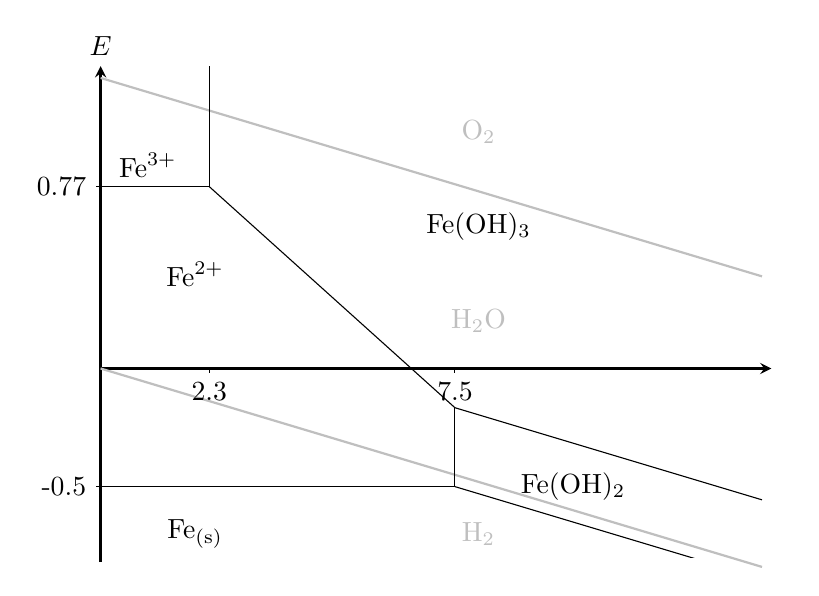
\begin{tikzpicture}[scale=0.6]
  \draw [thick, ->, >=stealth] (0,-4.1) -- (0,6.4) node[above]{$E$};
  \draw [thick, ->, >=stealth] (0,0) -- (14.2,0) node[above right]{$\pH$}; 
  %E-pH de l'eau
  \draw[thick, gray!50] (0, 1.23*5) -- ++(14, -0.3*14); 
  \draw[thick, gray!50] (0, 0) -- ++(14, -0.3*14); 
  \draw[] (8, 1) node[gray!50]{\ce{H2O}};
  \draw[] (8, 5) node[gray!50]{\ce{O2}};
  \draw[] (8, -3.5) node[gray!50]{\ce{H2}};

  %E-pH du Fer
  \draw (0,-2.5) -- (7.5,-2.5);
  \draw (0,7.7/2) -- (2.3,7.7/2);
  \begin{scope}
    \clip (0,-4) rectangle (14,6.4);
    \draw[scale=1,domain=7.5:14,variable=\x] plot ({\x},{-2.5-0.3*(\x-7.5)});
    \draw[scale=1,domain=7.5:14,variable=\x] plot ({\x},{7.7/2-0.9*(7.5-2.3)-0.3*(\x-7.5)});
    \draw[scale=1,domain=2.3:7.5,variable=\x] plot ({\x},{7.7/2-0.9*(\x-2.3)});
    \draw (2.3,7.7/2) -- (2.3,6.4);
  \end{scope}
  \draw (2,2) node{\ce{Fe^2+}};
  \draw (2,-3.5) node{$\ce{Fe}_{(\mathrm{s})}$};
  \draw (7.5,-2.5) -- (7.5,{7.7/2-0.9*(7.5-2.3)});
  \draw (10,-2.5) node{\ce{Fe(OH)2}};
  \draw (1,4.3) node{\ce{Fe^3+}};
  \draw (8,3.0) node{\ce{Fe(OH)3}};
  \draw (0, 0.77*5) -- ++(-0.1, 0) node[left]{ \num{0.77}};
  \draw (0, -0.5*5) -- ++(-0.1, 0) node[left]{ \num{-0.5}};
  \draw (2.3, 0) -- ++(0, -0.1) node[below]{ \num{2.3}};
  \draw (7.5, 0) -- ++(0, -0.1) node[below]{ \num{7.5}};
\end{tikzpicture}  
\captionof{figure}{Diagramme potentiel-pH du fer, sur lequel on a superposé le diagramme de l'eau}
\label{fig:fer}
\end{center}

\subsection{Utilisation du diagramme E-pH}%
\label{sub:utilisation_du_diagramme_e_ph}

Une espèce chimique qui ne dispose pas d'un domaine de stabilité (prédominance) commun avec l'eau, réagit pour donner des espèces compatibles. Par exemple sur la figure~\ref{fig:fer} on voit que le domaine d'existence du fer solide (\ce{Fe}) est disjoint du domaine de prédominance de \ce{H2O}. Le fer va donc être oxydé par l'eau. Par exemple à un $\pH< \num{7.5}$, on aura la réaction :
\begin{equation}
  \ce{Fe(s) + 2H+(aq) -> Fe^2+(aq) + H2(g)}
\end{equation}
Les oxydes de fer \ce{Fe(OH)2} et \ce{Fe(OH)3} ont un domaine d'existence commun avec celui de l'eau, ils sont stables dans l'eau.

\textbf{Attention :} une réaction qui est thermodynamiquement favorisée (le diagramme prévoit qu'elle se produise) peut être très lente et on peut observer des espèces instables en solution aqueuses. Exemples : eau oxygénée, eau de javel.

\subsection{Stabilité d'une espèce : dismutation}%
\label{sub:stabilite_d_une_espece_dismutation}

Déterminons le diagramme potentiel-pH de l'iode, en solution aqueuse, on peut avoir les espèces suivantes : \ce{I2}($no=0$), \ce{I-}($no = -\text{I}$), \ce{IO3-}($no=+\text{V}$) et donc le diagramme de situation suivant :
\begin{center}
  \begin{tikzpicture}
    \draw[-latex] (0,0) -- ++(4,0) node[right]{pH};
    \draw[-latex] (0,0) -- ++(0,3) node[right]{no};
    \draw (0,1) -- ++(4,0);
    \draw (0,2) -- ++(4,0);
    \draw (2, 0.5) node[]{\ce{I-}};
    \draw (2, 1.5) node[]{\ce{I2}};
    \draw (2, 2.5) node[]{\ce{IO3-}};
  \end{tikzpicture}
\end{center}
Et il faut déterminer les équations des deux frontières. On utilise une concentration de travail de $c_t=\SI{e-2}{\mol\per\litre}$. Cette fois nous considérerons comme convention de tracé qu'à une frontière entre deux espèces dissoutes, les concentrations des espèces sont égales et égales à la concentration de travail. 
\begin{itemize}
  \item \underline{\ce{I2 / I-} : }

  Demi-équation
  \begin{equation}
    \ce{I2(aq) + 2e- <=> 2I-(aq) }
  \end{equation}
  Formule de Nernst
  \begin{equation}
    E = E^\circ + \frac{\num{0.06}}{2} \log \left( \frac{[\ce{I2}]}{[\ce{I-}]^2} \right) = E^\circ + \num{0.06} = \SI{0.68}{\volt}
  \end{equation}

  \item \underline{\ce{IO3- / I2} :}

  Demi-équation
   \begin{equation}
     \ce{2IO3-(aq) +12H+(aq) + 10e- <=> I2(aq) + 6H2O(l)}
   \end{equation}
  Formule de Nernst
  \begin{equation}
    E = E^\circ + \frac{\num{0.06}}{10} \log \left( \frac{[\ce{H+}]^{12}[\ce{IO3-}]^2}{[\ce{I2}]\cz^{13}} \right) 
  \end{equation}
  sur la frontière, on a $[\ce{IO3-}] = [\ce{I2}] = c_t = \SI{e-2}{\mol\per\litre}$. On a donc 
  \begin{equation}
    E = E^\circ - \frac{2}{10}\times\num{0.06} - \frac{12}{10}\times\num{0.06}\pH = \num{1.19} - \num{0.024} - \num{0.072} \pH = \num{1.17}-\num{0.072}\pH
  \end{equation}
\end{itemize}
Ce qui donne le diagramme suivant
\begin{center}
  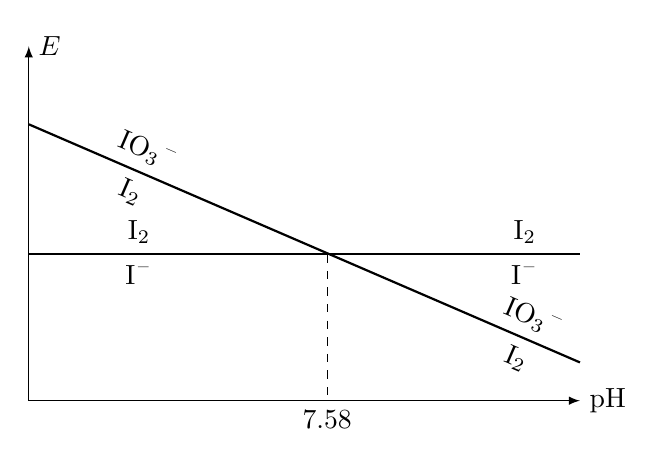
\begin{tikzpicture}
    \def\xscale{0.5}
    \def\yscale{3}
    \draw[-latex] (0,0) -- (14*\xscale,0) node[right]{pH};
    \draw[-latex] (0, 0) -- (0, 1.5*\yscale) node[right]{ $E$ };
    \draw[thick] (0, 1.17*\yscale) -- (14*\xscale, {(1.17-0.072*14)*\yscale}) 
    node[pos=0.2, above, sloped]{\ce{IO3-}}
    node[pos=0.2, below, sloped]{\ce{I2}}
    node[pos=0.9, above, sloped]{\ce{IO3-}}
    node[pos=0.9, below, sloped]{\ce{I2}};
    \draw[thick] (0, 0.62*\yscale) -- (14*\xscale, 0.62*\yscale)
    node[pos=0.2, above, sloped]{\ce{I2}}
    node[pos=0.2, below, sloped]{\ce{I-}}
    node[pos=0.9, above, sloped]{\ce{I2}}
    node[pos=0.9, below, sloped]{\ce{I-}};
    \draw[dashed] (\xscale*7.58, \yscale*0.62) -- ++(0, -\yscale*0.62) node[below]{\num{7.58}};

  \end{tikzpicture}
\end{center}
On observe qu'au delà de $\pH=\num{7.58}$, $\ce{I2}$ est présent dans deux domaines de prédominance disjoints, cela indique qu'il va réagir avec lui-même pour produire \ce{I-} et \ce{IO3-}, c'est une \textbf{dismutation}. Pour des pH supérieurs à \num{7.58} il ne peut plus y avoir de \ce{I2} et il ne reste plus qu'une frontière entre \ce{I-} et \ce{IO3-} qu'il faut déterminer.

\begin{itemize}
  \item \underline{\ce{IO3- / I-} : }

  Demi-équation
  \begin{equation}
    \ce{IO3- + 6H+ + 6e- <=> I- + 3H2O}
  \end{equation}
  Formule de Nernst
  \begin{equation}
    E = E^\circ + \frac{\num{0.06}}{6} \log \left( \frac{[\ce{H+}]^6[\ce{IO3-}]}{[\ce{I-}]\cz^6} \right) = E^\circ - \num{0.06}\pH 
  \end{equation}
  On a donc une frontière de pente \SI{-0.06}{\volt}
\end{itemize}
Et on obtient le diagramme suivant

\begin{center}
  \begin{tikzpicture}
    \def\xscale{0.5}
    \def\yscale{3}
    \draw[-latex] (0,0) -- (14*\xscale,0) node[right]{pH};
    \draw[-latex] (0, 0) -- (0, 1.5*\yscale) node[right]{ $E$ };
    \draw[thick] (0, 1.17*\yscale) -- (7.58*\xscale, {(1.17-0.072*7.58)*\yscale});
    \draw[thick] (0, 0.62*\yscale) -- (7.58*\xscale, 0.62*\yscale);
    \draw[thick] (7.58*\xscale, {(1.17-0.072*7.58)*\yscale}) -- ++({(14-7.58)*\xscale}, {-0.06*(14-7.58)*\yscale}); 
    \draw[dashed] (\xscale*7.58, \yscale*0.62) -- ++(0, -\yscale*0.62) node[below]{\num{7.58}};
    \draw (\xscale*3, \yscale*0.3) node{\ce{I-}}; 
    \draw (\xscale*2, \yscale*0.85) node{\ce{I2}}; 
    \draw (\xscale*8, \yscale*1.0) node{\ce{IO3-}}; 
  \end{tikzpicture}
\end{center}

\end{document}
